\begin{figure}[H]
    \centering
    \definecolor{deformblue}{RGB}{40,115,185}
    \definecolor{initialgray}{RGB}{115,120,125}
    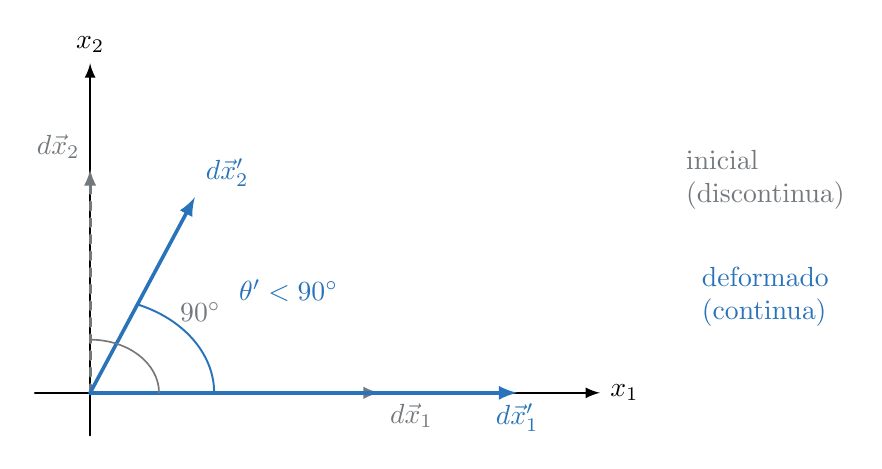
\begin{tikzpicture}[x=3.5cm,y=2.7cm,line cap=round,line join=round]
        \coordinate (O) at (0,0);
        \draw[-latex,line width=0.8pt] (-0.2,0) -- (1.85,0) node[right] {$x_1$};
        \draw[-latex,line width=0.8pt] (0,-0.2) -- (0,1.55) node[above] {$x_2$};

        \draw[initialgray,dashed,line width=1pt,-latex] (O) -- (1.05,0)
            node[below right] {$d\vec{x}_1$};
        \draw[initialgray,dashed,line width=1pt,-latex] (O) -- (0,1.05)
            node[above left] {$d\vec{x}_2$};

        \draw[deformblue,line width=1.3pt,-latex] (O) -- (1.55,0)
            node[below] {$d\vec{x}'_1$};
        \draw[deformblue,line width=1.3pt,-latex] (O) -- (0.38,0.92)
            node[above right] {$d\vec{x}'_2$};

        \draw[initialgray,line width=0.6pt] (0.25,0) arc[start angle=0,end angle=90,radius=0.25];
        \node[initialgray] at (0.4,0.38) {$90^\circ$};
        \draw[deformblue,line width=0.7pt] (0.45,0) arc[start angle=0,end angle=68,radius=0.45];
        \node[deformblue] at (0.72,0.48) {$\theta'<90^\circ$};

        \node[initialgray,align=left] at (2.45,1.0) {inicial\\(discontinua)};
        \node[deformblue,align=left] at (2.45,0.45) {deformado\\(continua)};
    \end{tikzpicture}
    \caption{Elementos materiales en el punto considerado, antes y después de la deformación.}
\end{figure}